\documentclass{article}

% if you need to pass options to natbib, use, e.g.:
%     \PassOptionsToPackage{numbers, compress}{natbib}
% before loading neurips_2019

% ready for submission
% \usepackage{neurips_2019}

% to compile a preprint version, e.g., for submission to arXiv, add add the
% [preprint] option:
    % \usepackage[preprint]{neurips_2019}

% to compile a camera-ready version, add the [final] option, e.g.:
\usepackage[final]{neurips}

% to avoid loading the natbib package, add option nonatbib:
    % \usepackage[nonatbib]{neurips_2019}
\usepackage{multicol}
\usepackage{float}
\usepackage[center]{caption}

\usepackage[utf8]{inputenc} % allow utf-8 input
\usepackage[T1]{fontenc}    % use 8-bit T1 fonts
\usepackage{hyperref}       % hyperlinks
\usepackage{url}            % simple URL typesetting
\usepackage{booktabs}       % professional-quality tables
\usepackage{amsfonts}       % blackboard math symbols
\usepackage{nicefrac}       % compact symbols for 1/2, etc.
\usepackage{microtype}      % microtypography
\usepackage{graphicx}
\usepackage{amsmath}
\usepackage{xepersian}

\settextfont{XB Yas.ttf}

\title{تکلیف شماره 7
 - 
 \lr{Mutual Exclusion}}


% The \author macro works with any number of authors. There are two commands
% used to separate the names and addresses of multiple authors: \And and \AND.
%
% Using \And between authors leaves it to LaTeX to determine where to break the
% lines. Using \AND forces a line break at that point. So, if LaTeX puts 3 of 4
% authors names on the first line, and the last on the second line, try using
% \AND instead of \And before the third author name.

\author{%
  امیرحسین مهدی‌نژاد\\
  شماره دانشجویی 810800058\\
  \texttt{mahdinejad@ut.ac.ir} \\
  % examples of more authors
  % \And
  % Coauthor \\
  % Affiliation \\
  % \texttt{email} \\
  % \AND
  % Coauthor \\
  % Affiliation \\
  % Address \\
  % \texttt{email} \\
}

% create title (includes both anonymized and non-anonymized versions)
% \providecommand{\@makepertitle}{}
% \newcommand{\makepertitle}{%
%   \vbox{%
%     \hsize\textwidth
%     \linewidth\hsize
%     \vskip 0.1in
%     \toptitlebar
%     \centering
%     {\LARGE\bf \@title\par}
%     \bottomtitlebar
%       \def\And{%
%         \end{tabular}\hfil\linebreak[0]\hfil%
%         \begin{tabular}[t]{c}\bf\rule{\z@}{24\p@}\ignorespaces%
%       }
%       \def\AND{%
%         \end{tabular}\hfil\linebreak[4]\hfil%
%         \begin{tabular}[t]{c}\bf\rule{\z@}{24\p@}\ignorespaces%
%       }
%       \begin{tabular}[t]{c}\bf\rule{\z@}{24\p@}\@author\end{tabular}%
%     \vskip 0.3in \@minus 0.1in
%   }
% }

\begin{document}


\begin{minipage}{0.1\textwidth}% adapt widths of minipages to your needs

\includegraphics[width=1.1cm]{Photos/UT_logo.png}
\end{minipage}%
\hfill%
\begin{minipage}{0.9\textwidth}\raggedleft
دانشکده فنی، دانشگاه تهران\\
سیستم‌های توزیع شده - 
دی
ماه 1400\\
\end{minipage}
% \end{}

\makepertitle

% ----------------------------------------------------------------------

% \begin{abstract}
%  این بخش از یک پاراگراف تشکیل شده است که توضیحاتی کلی در مورد مساله و راه حل شما ارائه می‌دهد.
% \end{abstract}
\begin{multicols}{2}
\section{}
الگوریتم میکاوا می‌تواند به بن‌بست بخورد. چرا که ممکن است یک سایت توسط سایت‌های دیگر قفل شده و در عین حال
\lr{request}
های بعدی با توجه به
\lr{timestamp}
اولویت پیدا نکنند و زنجیره‌ی این انتظار پاره نشود. به عبارت دیگر یک سایت ممکن است پیام
\lr{reply}
به سایتی ارسال کند و بعدا یک درخواست با اولویت بالاتر از یک سایت دیگر را مجبور به صبر کند.

فرض کنیم سه سایت
$S_i, S_j, S_k$
به طور همزمان فراخوانی انجام دهند و داشته باشیم:
$$R_i \cap R_j = \{ S_{ij} \}$$
$$R_j \cap R_k = \{ S_{jk} \}$$
$$R_k \cap R_i = \{ S_{ki} \}$$
از آنجایی که سایت‌ها پیام‌های
\lr{request}
را به ترتیب خاصی ارسال نمی‌کنند و تاخیر پیام‌ها دلخواه است، می‌توان این سناریو را در نظر گرفت:
$S_{ij}$
توسط
$S_i$
قفل شده، همچنین
$S_{jk}$
توسط
$S_j$
و به همین ترتیب
$S_{ki}$
توسط
$S_k$
قفل شده باشد. این حالت نشان‌دهنده‌ی بن‌بستی شامل سایت‌های
$S_i, S_j, S_k$
بوده و به عبارتی حلقه‌ی انتظار چرخشی به وجود آمده است، یعنی منتظر تایید یکدیگر می‌مانند.
\begin{figure}[H]
    \centering
    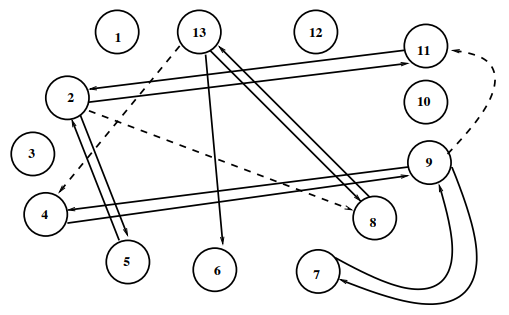
\includegraphics[width=0.90\linewidth]{Photos/HW7/deadlock.png}
    \caption{
    یک بن‌بست محتمل برای مثال داخل اسلایدها
    }
    \label{fig:my_label}
\end{figure}
در شکل فوق نقطه‌چین‌ها نشان‌دهنده‌ی انتظار است. ۲ برای ۸، ۹ برای ۱۱ و ۱۳ برای ۴ در این حالت باقی می‌مانند چرا که ۵ و ۱۱ توسط ۲، همچنین ۶ و ۸ توسط ۱۳ و به همین ترتیب ۴ و ۷ توسط ۹ قفل شده‌اند.\\
\rule{\linewidth}{1pt}
\section{}
بهترین توپولوژی برای الگوریتم ریموند، توپولوژی
\lr{radiating star}
است که در شکل ذیل نمونه‌ای از آن مشاهده می‌شود:
\begin{figure}[H]
    \centering
    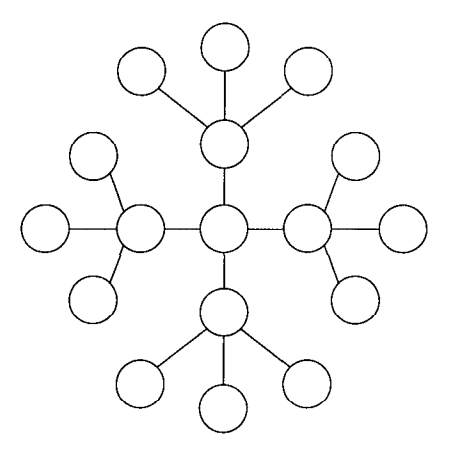
\includegraphics[width=0.50\linewidth]{Photos/HW7/radiatingStar.png}
    \caption{
    \lr{Radiating star topology}
    }
    \label{fig:my_label}
\end{figure}
اگر ظرفیت هر نود غیربرگ
$K$
باشد، در این صورت قطر درخت برابر است با:
$$2\left[ \log_{K-1}{\left(\frac{(N-1)(K-2)}{K}+1\right)} \right]$$
لذا بدترین حالت برای این توپولوژی
$O(\log_{K-1}{N})$
خواهد بود که از
$O(\sqrt{N})$
که در میکاوا داشتیم بهتر است.

لازم به ذکر است که قطر درخت با افزایش ظرفیت کاهش می یابد. لذا درخت‌هایی با
\lr{fanout}
بیشتر را بیشتر ترجیح می‌دهیم.

وقتی همه‌ی نودها
\lr{privilege}
می‌فرستند، این پیغام بین
$N-1$
یال در درخت، دقیقا دو بار رد و بدل می‌شود تا همه‌ی
$N$
نود از آن مطلع شوند و هرکدام از آن‌ها
\lr{response}
نیز در پی دارد که یعنی در مجموع
$4(n-1)$
پیام در طول درخت جابجا می‌شود.

در حقیقت رد و بدل کردن ۴ پیام برای هر اجرای
\lr{CS}
کافیست.
$$\frac{4(N-1)}{N} \approx 4$$
\begin{figure}[H]
    \centering
    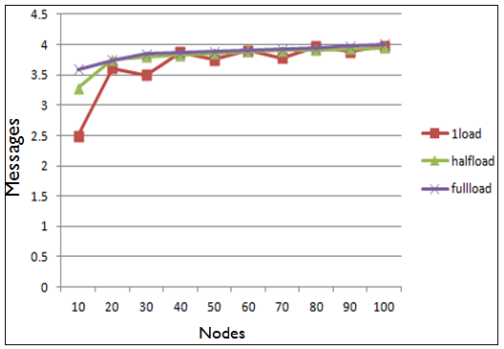
\includegraphics[width=0.99\linewidth]{Photos/HW7/chart.png}
    \caption{
    بررسی تعداد پیام‌ها در زنجیره‌ای از اجراهای الگوریتم ریموند در شرایط مختلف با توپولوژی
    \lr{Radiating star}
    }
    \label{fig:my_label}
\end{figure}
برای بدست آمدن نمودار شکل فوق، الگوریتم ۱۰ بار اجرا شده و میانگین تعداد پیام‌هایی که در هر فراخوان
\lr{Critical Section}
ارسال شده را محاسبه کرده‌اند.
\end{multicols}
\end{document}
